\documentclass[12pt,letterpaper]{article}
\usepackage{amsmath,amsthm,amsfonts,amssymb,amscd}
\usepackage{listings}
\usepackage{color}
\usepackage{rotating}

\definecolor{dkgreen}{rgb}{0,0.6,0}
\definecolor{gray}{rgb}{0.5,0.5,0.5}
\definecolor{mauve}{rgb}{0.58,0,0.82}

\lstset{%frame=tb,
  language=Bash,
  aboveskip=3mm,
  belowskip=3mm,
  showstringspaces=false,
  columns=flexible,
  basicstyle={\small\ttfamily},
  numbers=none,
  numberstyle=\tiny\color{gray},
  keywordstyle=\color{blue},
  commentstyle=\color{dkgreen},
  stringstyle=\color{mauve},
  breaklines=true,
  breakatwhitespace=true
  tabsize=3
}
%\usepackage{tabularx}
\usepackage{url}
\usepackage{caption}
\usepackage{subcaption}
\usepackage{graphicx}
\usepackage{wrapfig}
\usepackage{xcolor}
\usepackage[english]{babel}
\usepackage{mathtools}
\usepackage{fixltx2e}
\usepackage{hyperref}
\usepackage{enumerate}
\usepackage{fancyhdr}
\usepackage{mathrsfs}
\usepackage[margin=3cm]{geometry}
\setlength{\parindent}{0.0in}
\setlength{\parskip}{0.05in}

% Edit these as appropriate

\newcommand\course{CS595}
\newcommand\semester{Fall 2013}     
\newcommand\hwnum{9}
\newcommand\yourname{Amara Naas}
\newcommand\login{anaas}
\newcommand\DATE{12/5/2013}

\newenvironment{answer}[1]{
  \subsubsection*{Problem #1}
}

\pagestyle{fancyplain}
\headheight 40pt
\lhead{\yourname\ (\login)\\\course\ --- \semester}
\chead{\textbf{\Large Assignment \hwnum}}
\rhead{\DATE}
\headsep 40pt

\begin{document}
In my approach to attempt this assignment I used some functions which available at chapter three of our text book\cite{source} and used the {\it 100 blogs} from \cite{blogs}, including: 
\begin{itemize}
\item \url {http://f-measure.blogspot.com/feeds/posts/default}
\item \url {http://ws-dl.blogspot.com/feeds/posts/default}
\end{itemize}


as specified in assignment 9. I found that 17 out of the 100 blogs do not have the correct RSS blog so I had to replace them with the correct ones. {\it 17blogsListError.txt} shows these 17 blogs.
In order to solve the four problems in this assignment I created two python programs {\it Assignment9A.py}\footnote{File uploaded to github} and {\it Assignment9B.py}\footnotemark[1] which will solve problem 1 and problems 2-4 respectively.
\begin{answer}{1}
In first program I used two functions and the {\it list.txt}\footnotemark[1] file.
First {\it getwordcounts} function passes the summary or the description, that{\it RSS' list} of entries have, 
to the second {\it getwords} function and returns title and dictionary of word counts for an RSS feed.

For solving problem 1 the feeding list of 100 blogs and Assignment9A.py are used which will do the following:
\begin{itemize}
\item Looping over the feeds to read blogs from list.txt and generates the word counts for each blog and the number of blogs each word appeared in apcount dictionary.
\lstinputlisting[language=Python, firstline=32, lastline=47]{Assignment9A.py}

\item Sorting words in descending order, reducing their total number by maximum (50 \%) and minimum (10 \%) percentages, and filter out single letter words.

\lstinputlisting[language=Python, firstline=49, lastline=59]{Assignment9A.py}
\item Using the list of first 500 words and the list of blogs to create a text file called {\it BlogMatrix.txt} which contains a big matrix of all the word counts for each of the blogs.
\lstinputlisting[language=Python, firstline=63, lastline=78]{Assignment9A.py}

\end{itemize}

\end{answer}

\begin{answer}{2}

For problem two I used four function from \cite{source} as described in {\it Assignment9B.py}.
\begin{enumerate}

\item First {\it readfile} function will read list of words for each column-data, list of blogs names, and a big list of data where every item in the list is the data for that blog in particular row.

\lstinputlisting[language=Python, firstline=8, lastline=20]{Assignment9B.py}

\item For defining closeness a {\it pearson} correlation function is used because some blogs contain more entries or much
longer entries than others, and will thus contain more words overall. It tries to determine how well two sets of
data fit onto a straight line.

\lstinputlisting[language=Python, firstline=23, lastline=36]{Assignment9B.py}

\item The {\it bicluster} class is used because the cluster in a hierarchical clustering algorithm has some properties such
as being a point in the tree with two branches, or an endpoint associated with a blog, or contains data about its location.
\lstinputlisting[language=Python, firstline=38, lastline=44]{Assignment9B.py}
\item hierarchical function {\it hcluster} creates group of clusters as following:
\begin{enumerate}
\item Creates initial group clusters which are just the original items.
\lstinputlisting[language=Python, firstline=48, lastline=51]{Assignment9B.py}
\item Finding the two best matches of blogs to form the new single cluster until only one cluster is remains. 
\begin{flushleft}
\lstinputlisting[language=Python, firstline=52, lastline=77]{Assignment9B.py}
\end{flushleft}


\item This function uses pearson correlation and averaging the data for the two old clusters.
\item The final cluster returned by this function can be searched recursively to recreate all the clusters and their end nodes. 
\end{enumerate}
\item {\it printcluster} function writes all clusters to file called 
{\it Q2-ASCII.txt} using the recursive search.
\lstinputlisting[language=Python, firstline=78, lastline=93]{Assignment9B.py}
\item The {\it drawdendrogram} function uses the Python Imaging Library (PIL) which generates images with text and lines and save it in blogclust.jpg. This function dose the following:
\begin{enumerate}
\item Calls another recursive function called {\it getheight} which gives the total height of a given 
cluster. If the cluster is an endpoint, then its height is 1; otherwise, its height is the sum of the heights
of its branches.
\lstinputlisting[language=Python, firstline=96, lastline=102]{Assignment9B.py}
\item It also calls another recursive function called {\it getdepth} which returns the distance (The total error of the root node)
of an endpoint or the max distance of a branch.
\lstinputlisting[language=Python, firstline=104, lastline=110]{Assignment9B.py}
\item It has a scaling factor which determined by dividing the
fixed width (1200) by the total depth returned from getdepth function.
\lstinputlisting[language=Python, firstline=112, lastline=118]{Assignment9B.py}
\item After it creates a draw object for this image it calls the {\it drawnode} function to be halfway down the left side of this image.
\lstinputlisting[language=Python, firstline=119, lastline=125]{Assignment9B.py}
\end{enumerate}
\item {\it drawnode} function takes a cluster and its location and draws lines one long vertical line 
and two horizontal lines for each child where the lengths of the horizontal lines show the similarity of clusters.
Shorter line indicate that clusters were almost identical.
\lstinputlisting[language=Python, firstline=127, lastline=147]{Assignment9B.py}

\end{enumerate}
\begin{figure}
        \center
                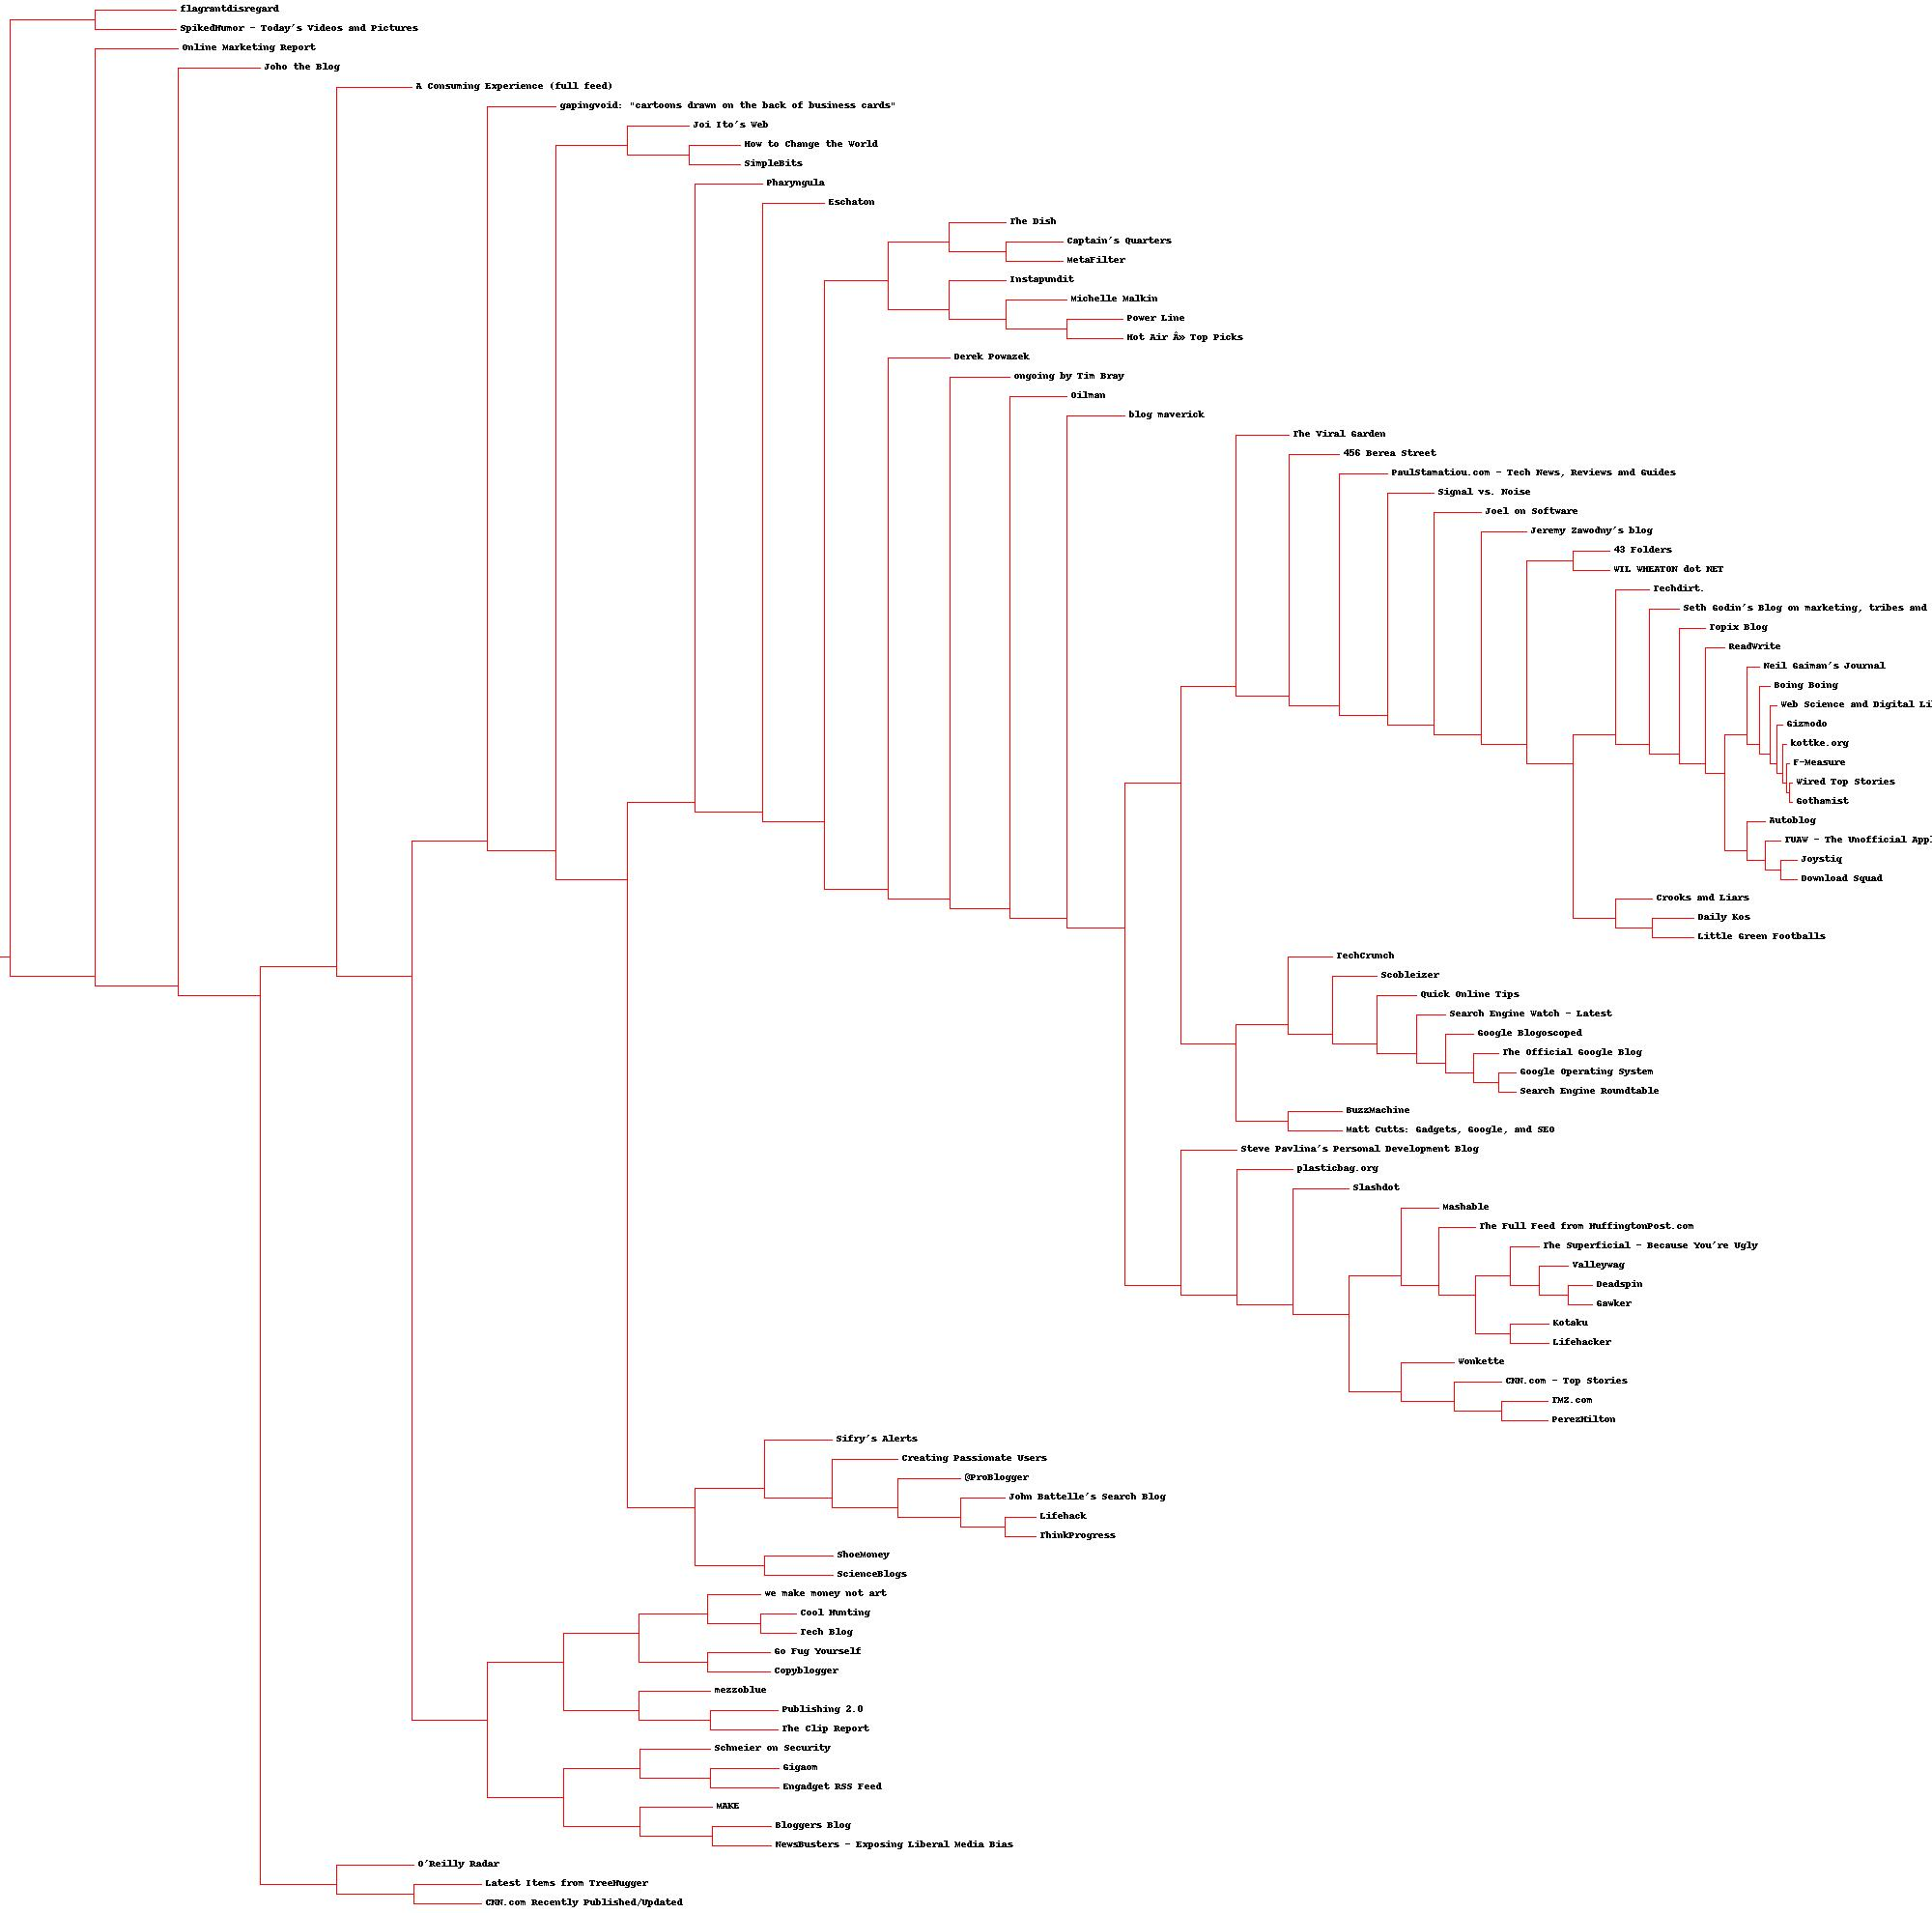
\includegraphics[width=\linewidth]{Clust_Dendrogram.jpg} 
        \caption{Dendrogram showing blog clusters}
       \label{fig:graph-before}
\end{figure}
\end{answer}

\begin{answer}{3}

I used kcluster function from \cite{source} to solve problem 3 which operates based on an algorithm called K-Means Clustering.
This algorithm breaks the data into distinct groups because it is told in advance how many distinct clusters to generate. this function dose the following:

\begin{itemize}

\item Takes the same data rows obtained from {\it readfile} function and the number of clusters {\it (k)} as an input.



\item Place a K points randomly in space that represent the centre of the cluster and assigns each blog to the nearest one.

\lstinputlisting[language=Python, firstline=151, lastline=155]{Assignment9B.py}

\item Moves centroids to the average location of all the nodes that assigned to them.

\lstinputlisting[language=Python, firstline=173, lastline=182]{Assignment9B.py}

\item Repeats this process until the assignments stop changing.
\lstinputlisting[language=Python, firstline=170, lastline=171]{Assignment9B.py}

\item Returns the k lists and the number of iterations it takes to produce the final result.


\end{itemize}

Table 1 shows the results when k is 5, 10, and 20.
\begin{table}[ht]

\centering

    \begin{tabular}{ c | c | c }
    \hline
    k=5 &  k=10 & k=20\\ \hline\hline
    
5   &  7 & 5 \\
    \hline
    \end{tabular}

\caption{The interations required for k=5,10,20}

\end{table}
\end{answer}
\begin{answer}{4}

For viewing data in two dimensions I used two functions {\it scaledown} and {\it draw2d} that obtained from \cite{source}. First function uses multidimensional scaling technique and does the following:

\begin{itemize}

\item Takes the data vector obtained from {\it readfile} function and finds the difference between each pair 
of blogs and matches them to a distances using Pearson correlation. These distances will represent 
the distances between the blogs in the chart.

\lstinputlisting[language=Python, firstline=185, lastline=198]{Assignment9B.py}

\item Every node representing a blog is moved according to the combination of all the other nodes pushing and pulling on it based on how close they are.

\lstinputlisting[language=Python, firstline=199, lastline=211]{Assignment9B.py}

\item This procedure is repeated many times until the distance cannot be reduced by moving the nodes any more.

\lstinputlisting[language=Python, firstline=215, lastline=216]{Assignment9B.py}

\item Returns the X and Y coordinates of the blogs on the two-dimensional chart. 

\end{itemize}
The second function uses use PIL to generate an image with all the labels of all the different blogs plotted at the coordinates of that blog which obtained from first function.

\lstinputlisting[language=Python, firstline=224, lastline=231]{Assignment9B.py}

\begin{figure}
        \center
                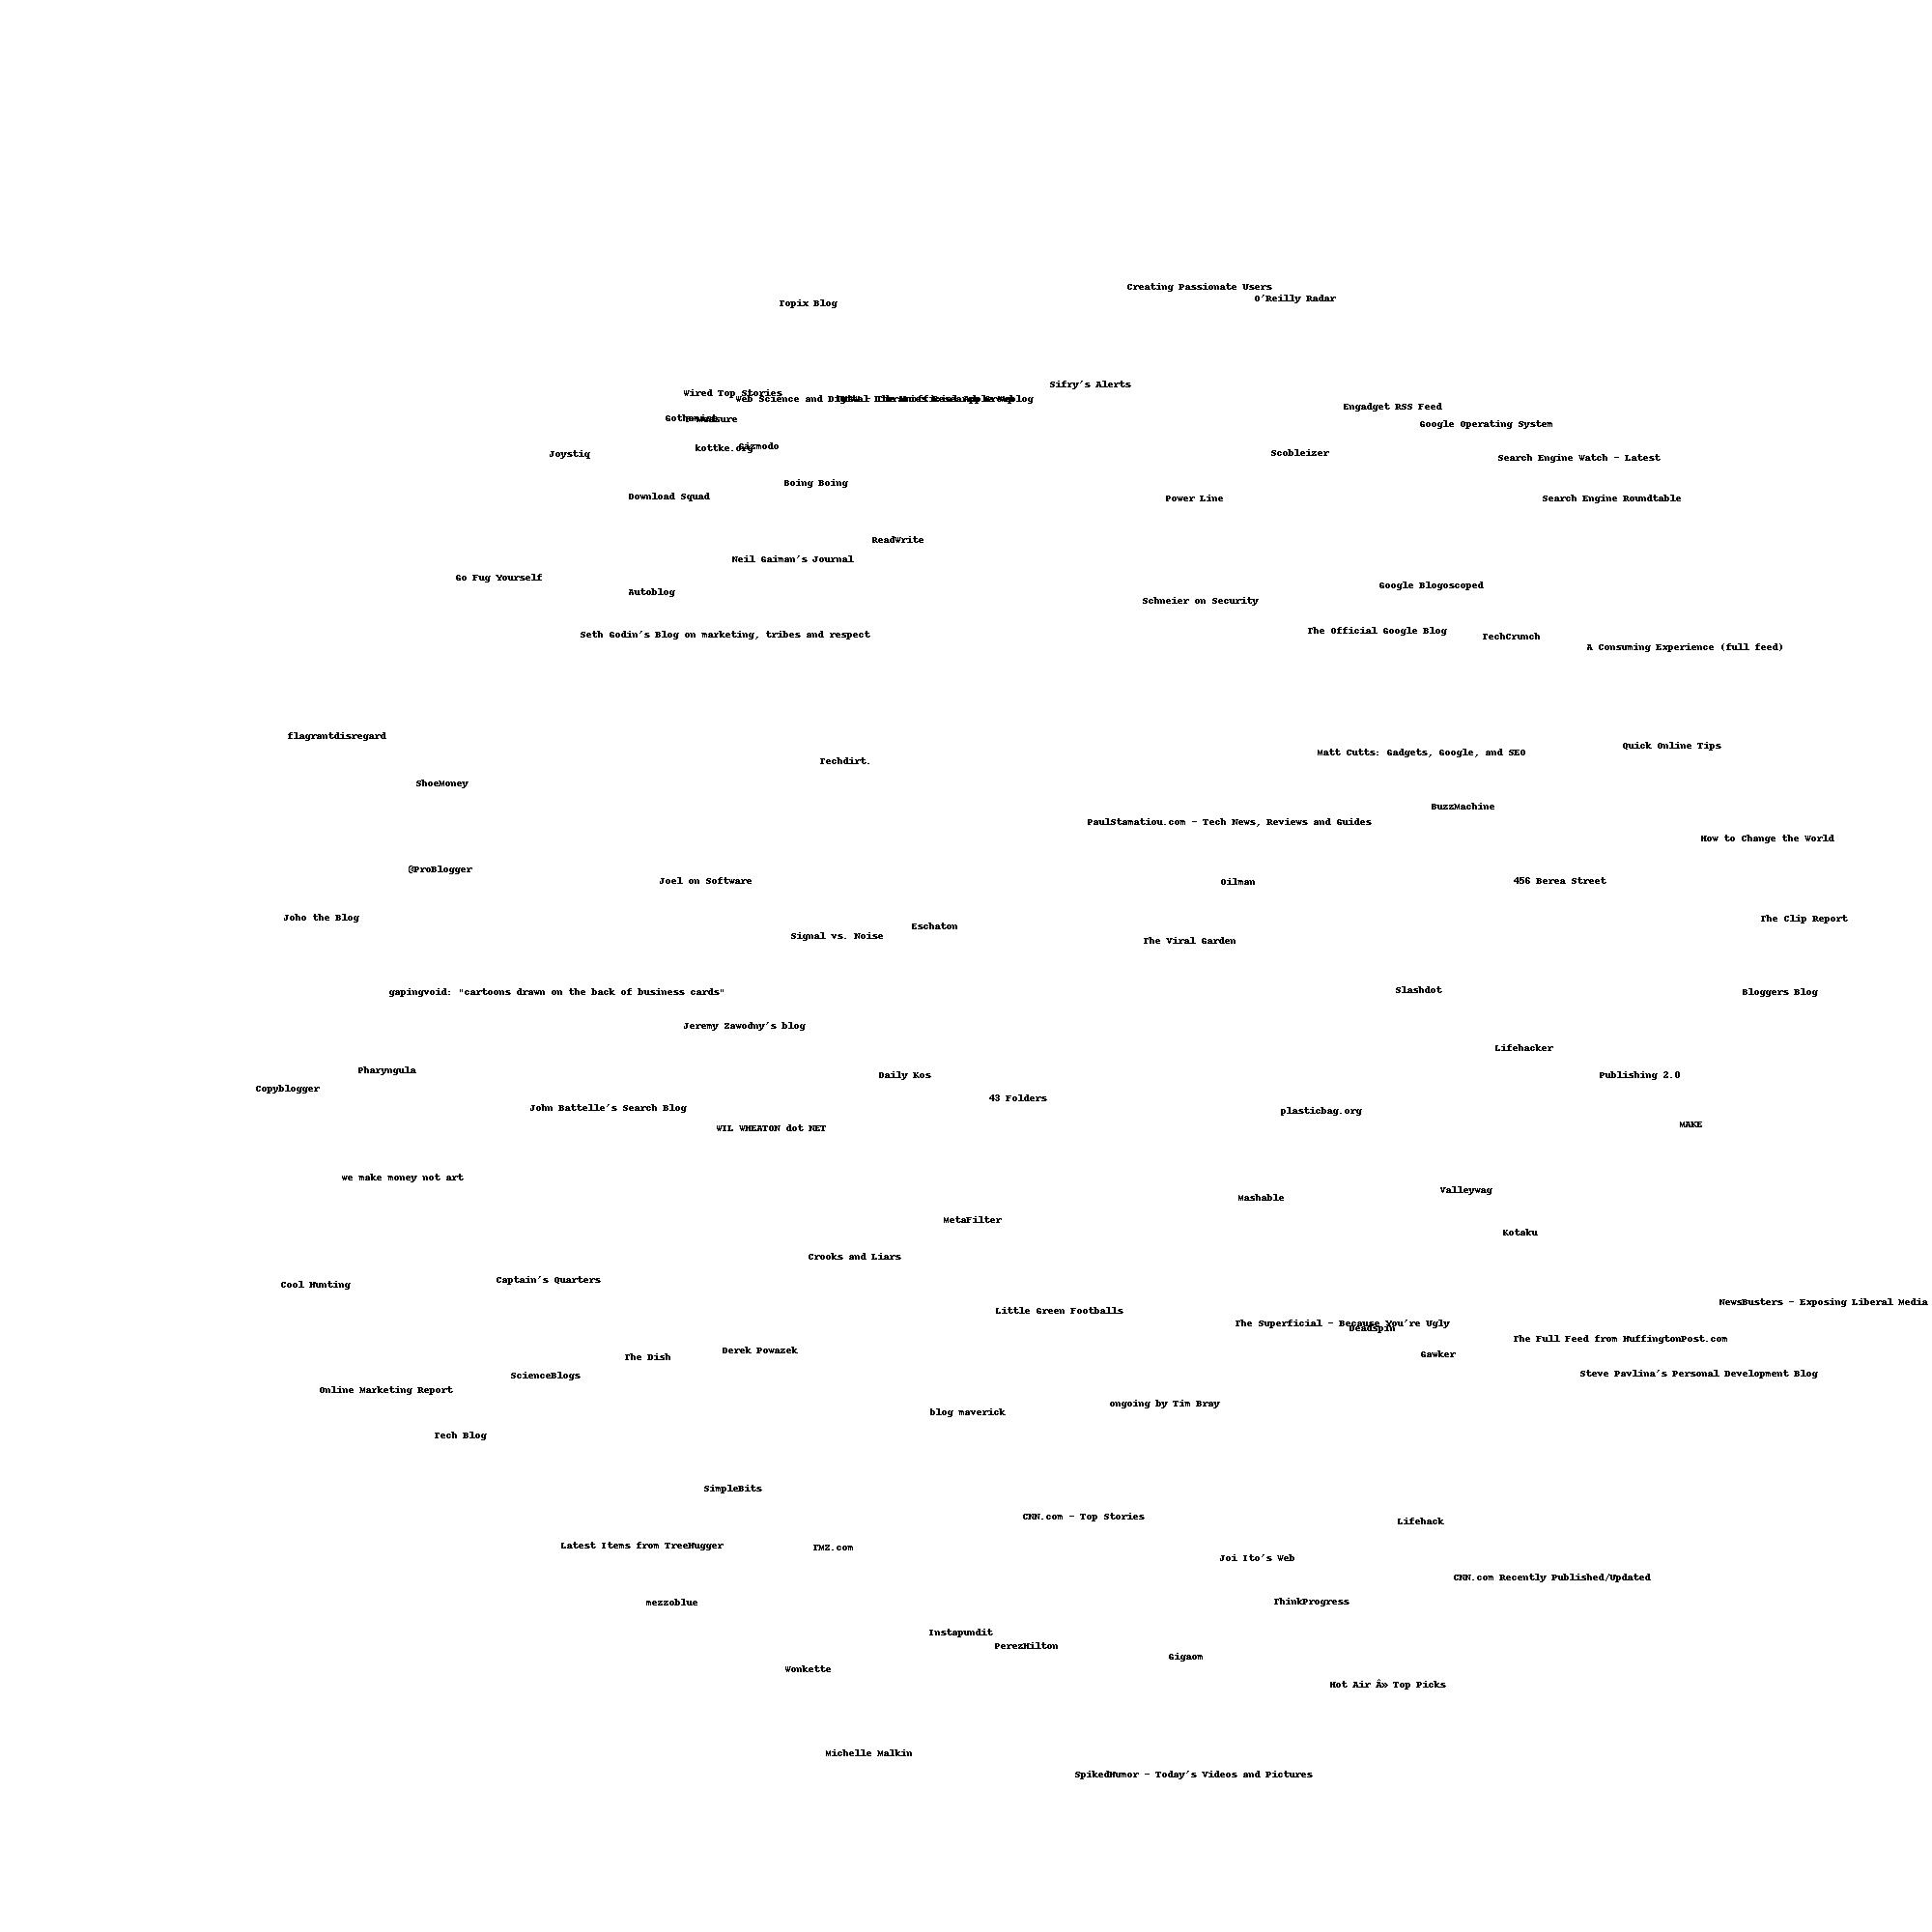
\includegraphics[width=\linewidth]{MDS.jpg} 
        \caption{2D representation of blog space}
       \label{fig:graph-before}
\end{figure}

\end{answer}
\begin{answer}{5}

For Creating an ASCII and JPEG dendrogram that clusters the most similar blogs using TFIDF calculations I made one change to the {\it Assignment9A.py} which is finding the total number of words in each count and run the code in {\it Assignment9X.py} to create the dendrogram. It seems that there are some changes due to the use of the same 500 words. Each time we parse the blogs we get different data and using TFIDF with the same words from question 2 increase the chances of a pair of blogs being different. Figure 4 and 5 show the ASCII and JPEG dendrogram.

\begin{figure}
        \center
                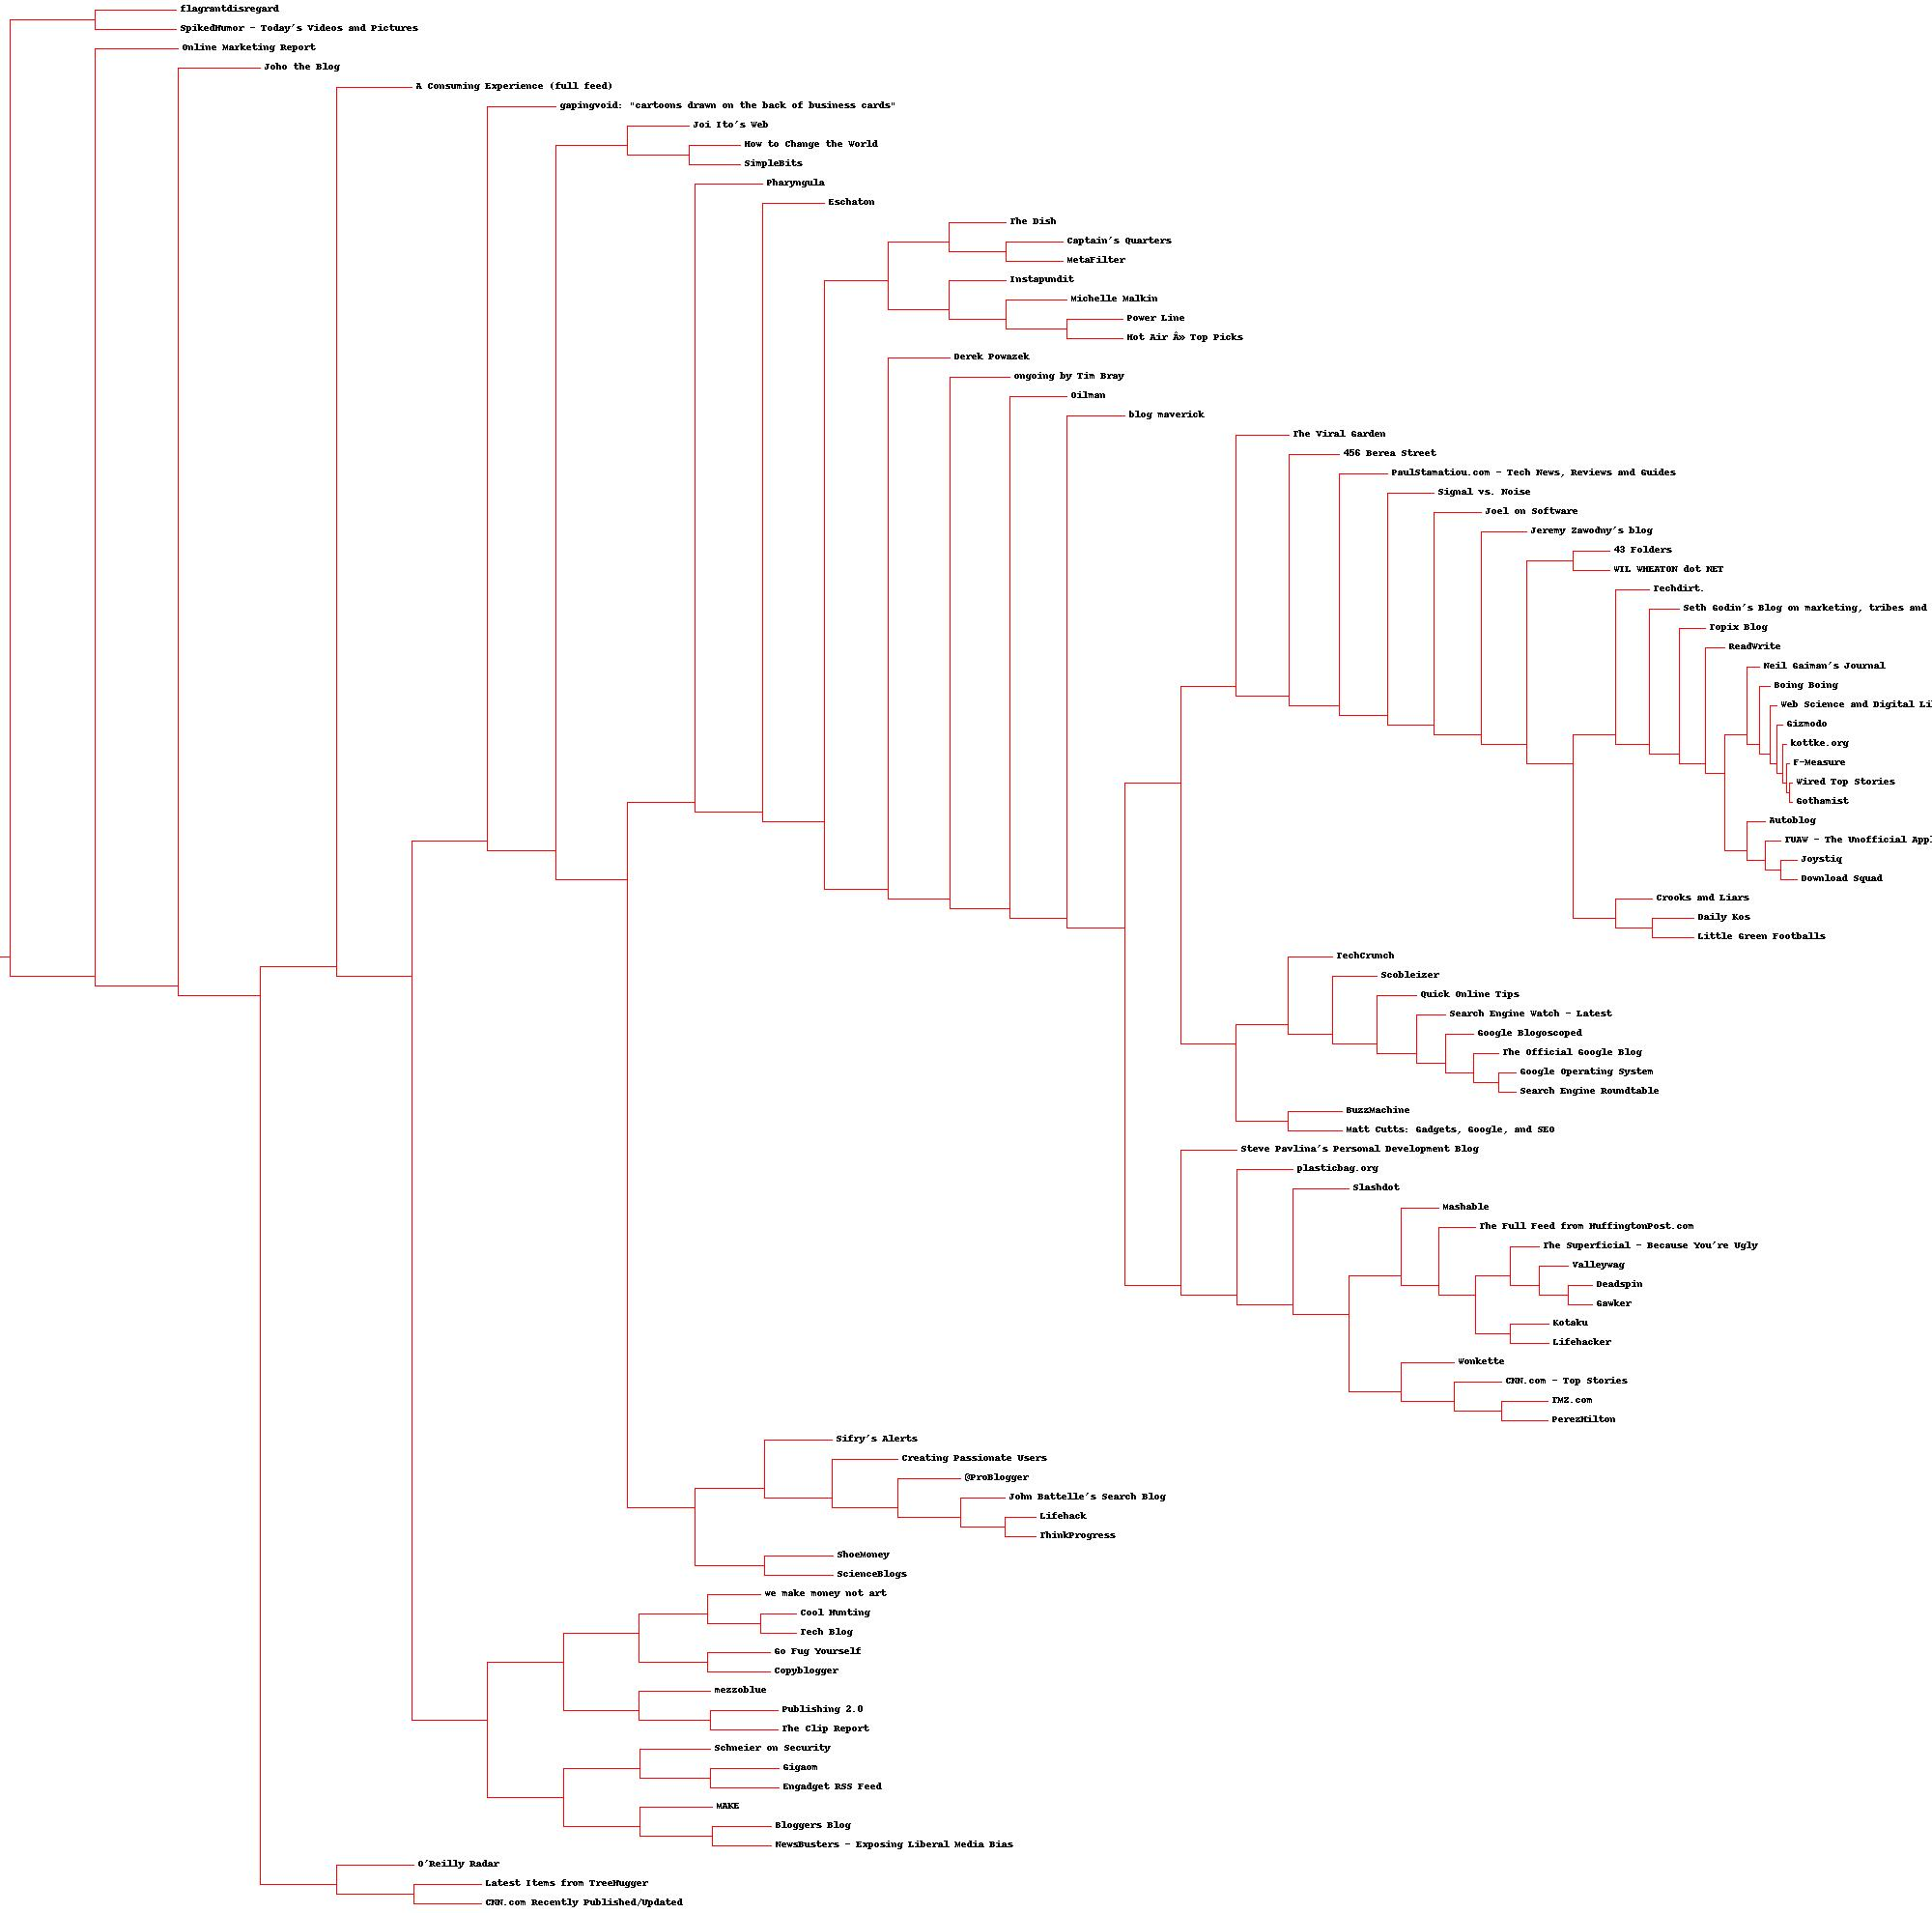
\includegraphics[width=\linewidth]{Clust_Dendrogram.jpg} 
        \caption{Dendrogram showing blog clusters using TFIDF}
       \label{fig:graph-before}
\end{figure}

\begin{figure}
        \center
                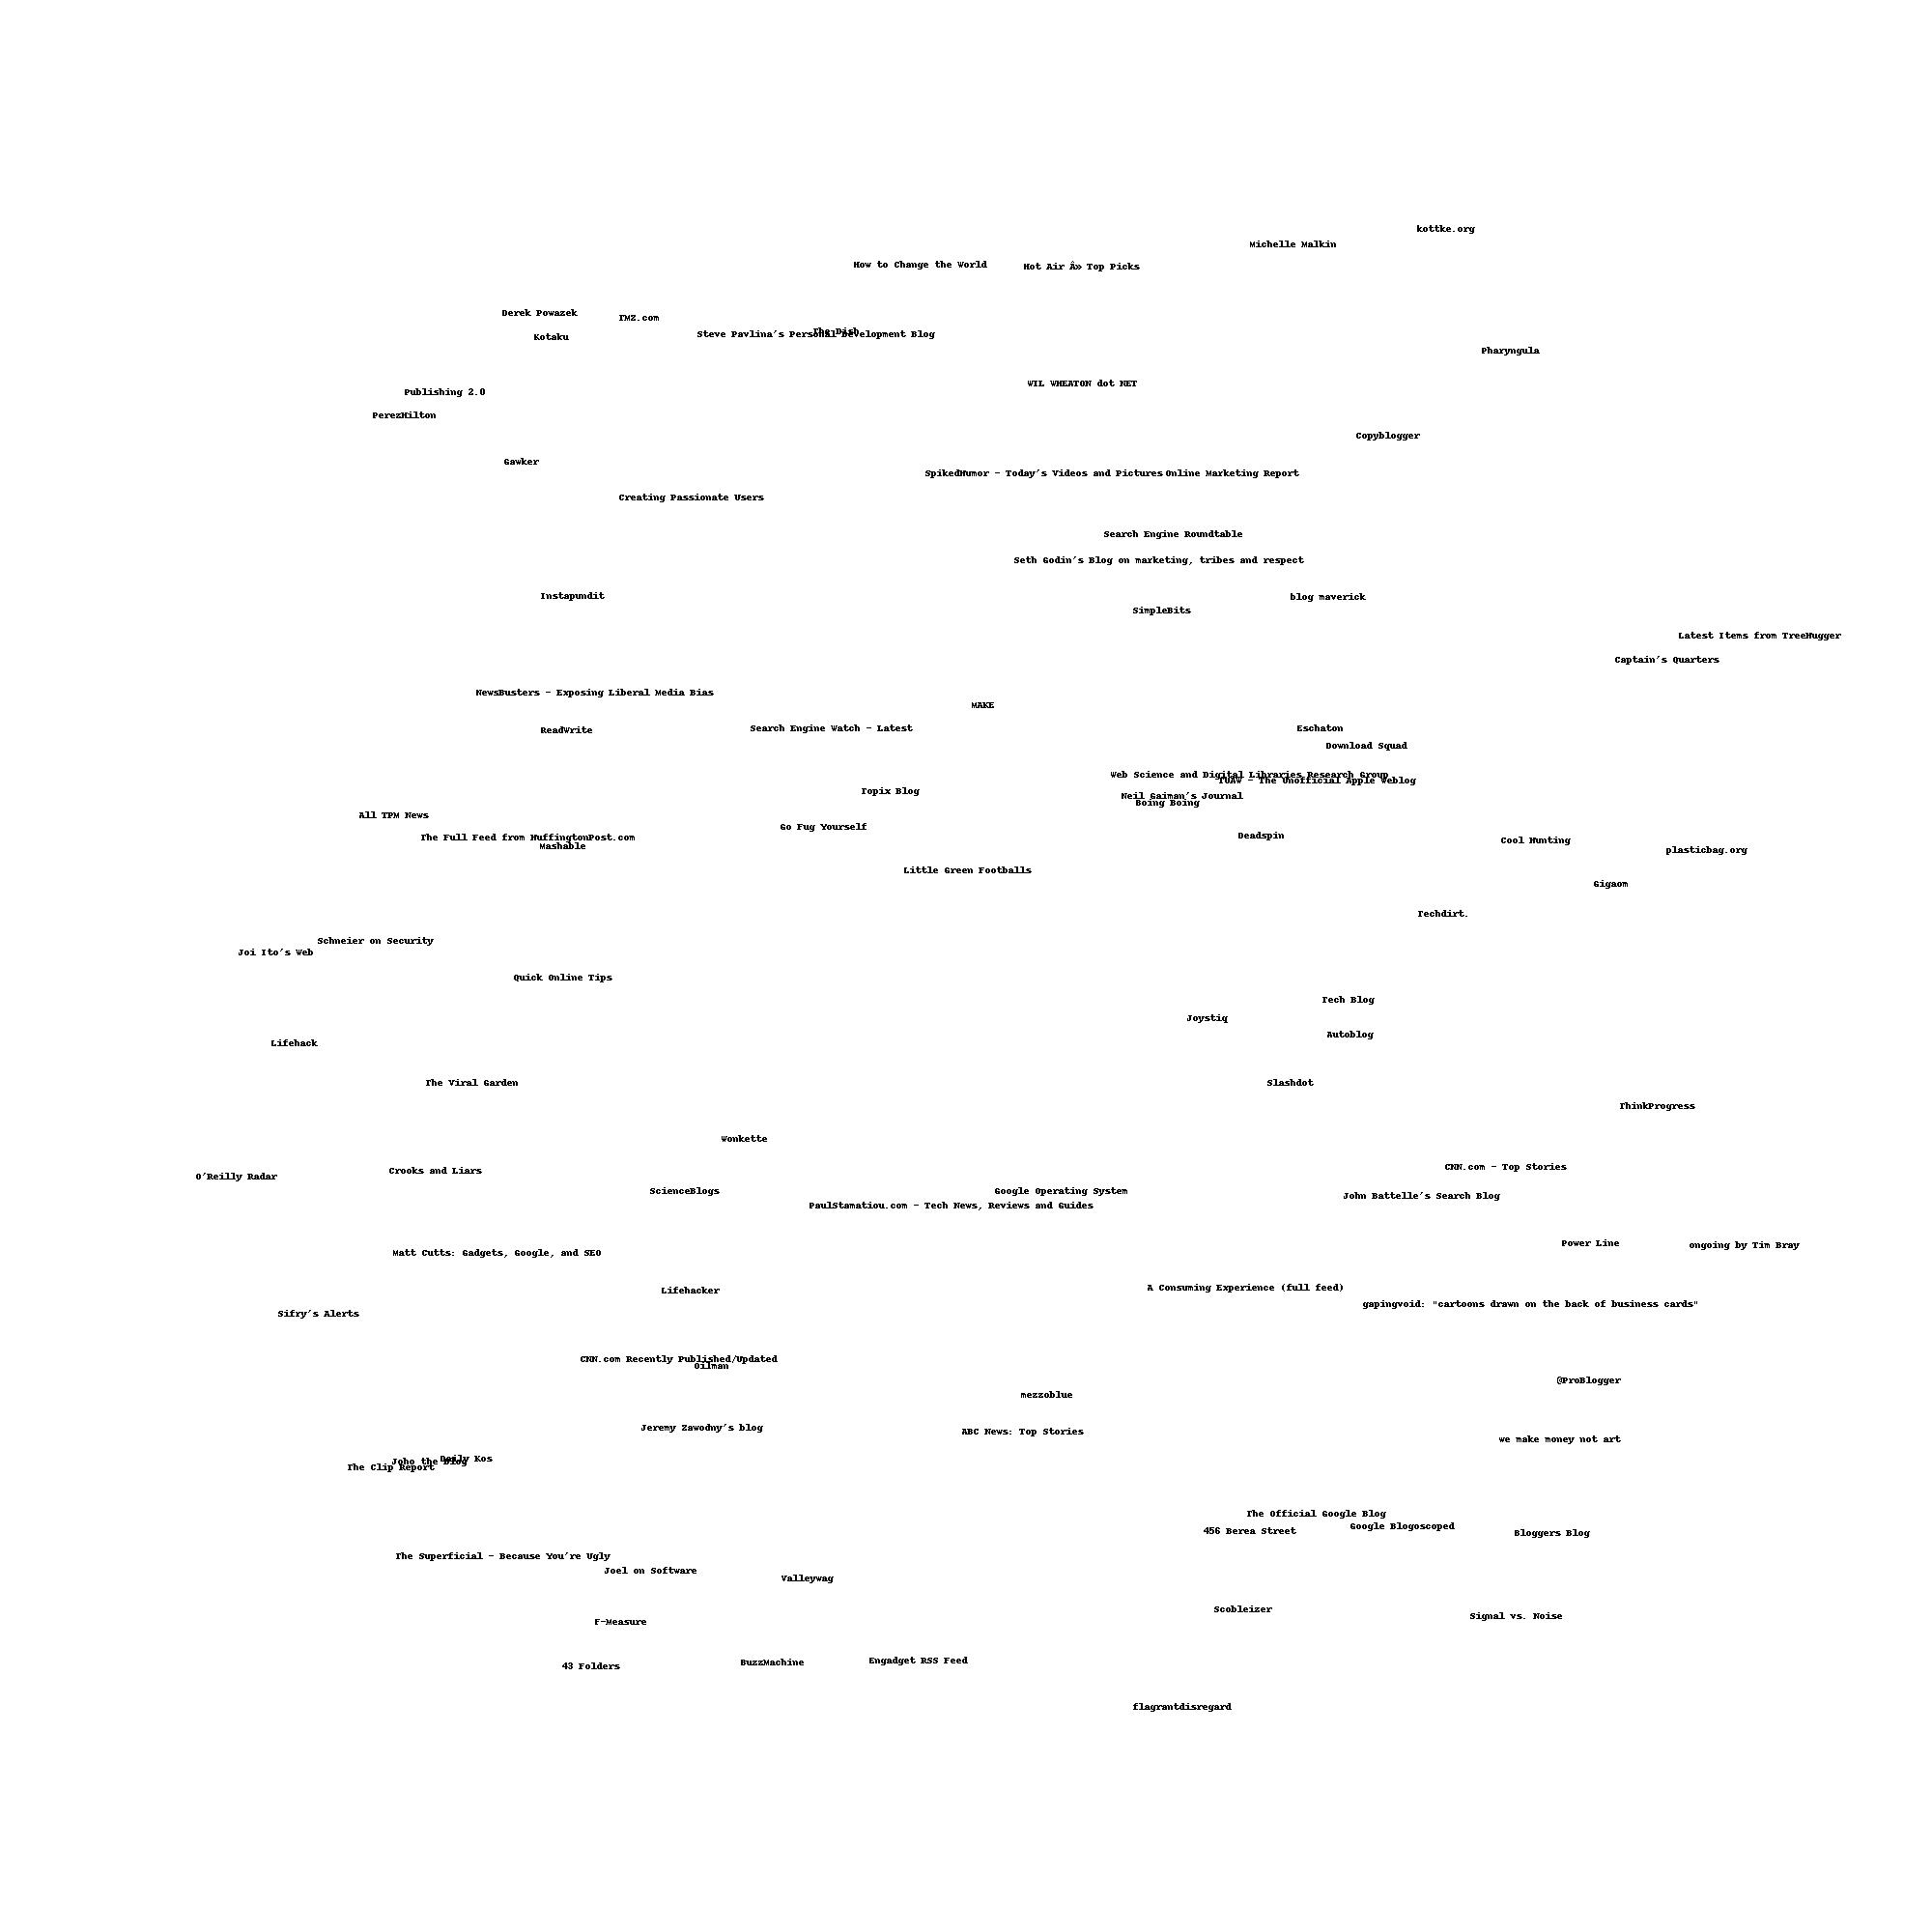
\includegraphics[width=\linewidth]{TFIDF_MDS.jpg} 
        \caption{2D representation of blog space using TFIDF}
       \label{fig:graph-before}
\end{figure}


\end{answer}

\clearpage
\bibliographystyle{plain}
\begin{thebibliography}{2}


\bibitem{source}
 T. Segaran, Discovering Groups, pp.~29--53 in: 
``Programming Collective Intelligence'', O'REILLY, Aug. 2007.

\bibitem{blogs}
 \url {https://github.com/nico/collectiveintelligence-book/blob/master/feedlist.txt}.
\end{thebibliography}

\end{document}